% !TEX root = ../../../main.tex
% 来源：中学数学实验教材·第三册（高中数学）
% 章节：二次函数 / 和二次函数有关的课题
% 原始文件：5.tex，行 1587-1615
% 类型：tikz
% ---
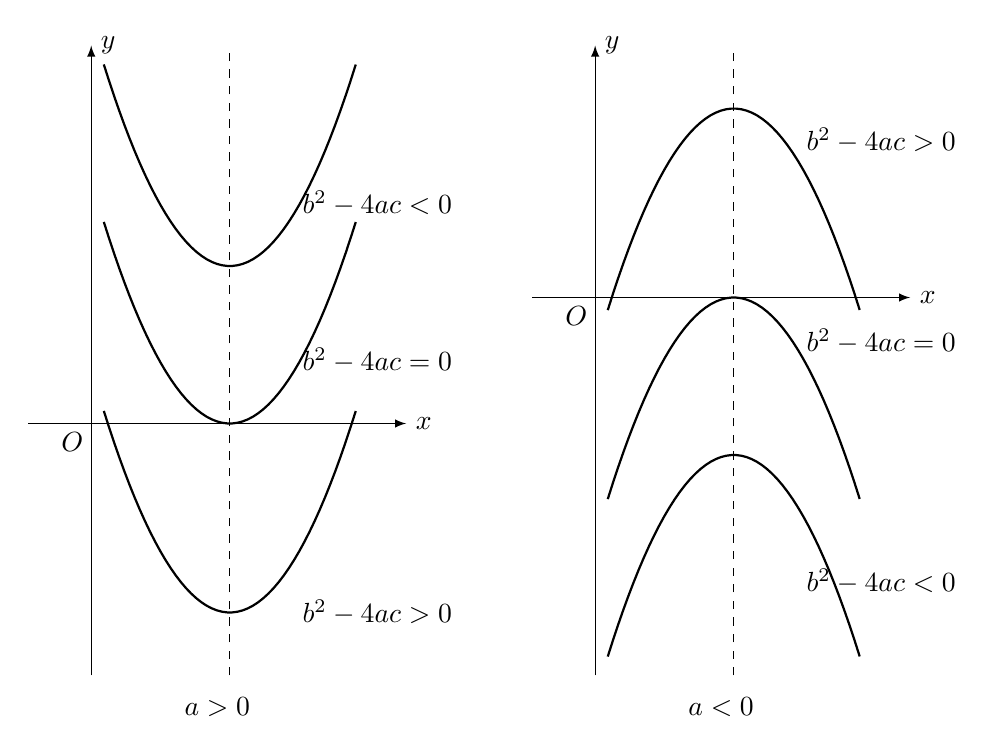
\begin{tikzpicture}[>=latex, scale=.8]
\begin{scope}
    \draw[->] (-1,0)--(5,0)node[right]{$x$};
    \draw[->] (0,-4)--(0,6)node[right]{$y$};
    \draw[domain=.2:4.2, samples=50, thick]plot(\x, {(\x-2.2)*(\x-2.2)*.8});
    \draw[domain=.2:4.2, samples=50, thick]plot(\x, {(\x-2.2)*(\x-2.2)*.8+2.5});
    \draw[domain=.2:4.2, samples=50, thick]plot(\x, {(\x-2.2)*(\x-2.2)*.8-3});
    \draw[dashed] (2.2,-4)--(2.2,6);
    \node at (-.3,-.3){$O$};
    \node at (2,-4.5){$a>0$};
\node at (3.2,-3)[right]{$b^2-4ac>0$};
\node at (3.2,1)[right]{$b^2-4ac=0$};
\node at (3.2,3.5)[right]{$b^2-4ac<0$};
\end{scope}

\begin{scope}[xshift=8cm, yshift=2cm]
    \draw[->] (-1,0)--(5,0)node[right]{$x$};
    \draw[->] (0,-6)--(0,4)node[right]{$y$};
    \draw[domain=.2:4.2, samples=50, thick]plot(\x, {-(\x-2.2)*(\x-2.2)*.8});
    \draw[domain=.2:4.2, samples=50, thick]plot(\x, {-(\x-2.2)*(\x-2.2)*.8-2.5});
    \draw[domain=.2:4.2, samples=50, thick]plot(\x, {-(\x-2.2)*(\x-2.2)*.8+3});
    \draw[dashed] (2.2,-6)--(2.2,4);
    \node at (-.3,-.3){$O$};
    \node at (2,-6.5){$a<0$};
    \node at (3.2,-4.5)[right]{$b^2-4ac<0$};
    \node at (3.2,-.7)[right]{$b^2-4ac=0$};
    \node at (3.2,2.5)[right]{$b^2-4ac>0$};
\end{scope}
\end{tikzpicture}
